\documentclass{article}
\usepackage{graphicx} % Required for inserting images
\usepackage{setspace} % Double Space 
\usepackage{ragged2e} % justify text
\usepackage{enumitem} % enumeration within subsection
\usepackage{url} % inserting links and urls

\usepackage{pdflscape} % Horizontal page orientation
\usepackage{booktabs}  % For \toprule, \midrule and \bottomrule
\usepackage{float} 

\usepackage[letterpaper, left=2cm, right=2cm, top=3cm, bottom=3cm]{geometry}

\setlength{\parskip}{1em} % we increase paragraph spacing

\title{Tesis}
\author{GUSTAVO ANDRES GONZALEZ PINEDA}
\date{February 2025}

\begin{document}

\begin{center}
\begin{doublespace}
    \thispagestyle{empty}  % no numbering for the cover
    \Large{UNIVERSIDAD DEL VALLE DE GUATEMALA}\\
    Facultad de Ingeniería \\
    Ingeniería en Ciencias de la Computación y Tecnologías de la Información 

    % Image placement
    \vspace{15mm} 
    
\includegraphics[width=0.2\textwidth]{images/Uvg_logo.jpg}

    \vspace{15mm} 
    {\Large Desarrollo de algoritmo de Pathfinding en Aplicación de recorridos virtuales con realidad aumentada para el Centro de Innovación y Tecnología de la Universidad del Valle de Guatemala.}

    \vspace{10mm} 
    {\Large Trabajo de graduación en modalidad de Megaproyecto presentado por Gustavo González
    para optar al grado academico de Licenciatura en Ingeniería en Ciencias de la Computación y Tecnologías de la Información.}

    {\Large Guatemala, \\ 2025}
    
\end{doublespace}
\end{center}

\newpage % page left purposely on blank

\thispagestyle{empty} % Remove headers and footers (optional)
\mbox{} % Ensure the page is not optimized away
\newpage % Move to the next page


\begin{center}
    \begin{doublespace}
        \thispagestyle{empty}  % no numbering for the cover
        \Large{UNIVERSIDAD DEL VALLE DE GUATEMALA}\\
        Facultad de Ingeniería \\
        Ingeniería en Ciencias de la Computación y Tecnologías de la Información 
    
        % Image placement
        \vspace{15mm} 
        
\includegraphics[width=0.2\textwidth]{images/Uvg_logo.jpg}
    
        \vspace{15mm} 
        {\Large Desarrollo de algoritmo de Pathfinding en Aplicación de recorridos virtuales con realidad aumentada para el Centro de Innovación y Tecnología de la Universidad del Valle de Guatemala.}
    
        \vspace{10mm} 
        {\Large Trabajo de graduación en modalidad de Megaproyecto presentado por Gustavo González
        para optar al grado academico de Licenciatura en Ingeniería en Ciencias de la Computación y Tecnologías de la Información.}
    
        {\Large Guatemala, \\ 2025}
        
    \end{doublespace}
    \end{center}


% end of cover section


\setcounter{page}{1} % Start page numbering from page 1

\section{Abstract}
{\justify This project aims to develop an augmented reality application for virtual tours within the campus of Universidad del Valle de Guatemala, integrating a precise navigation system using Estimote Beacons with Ultra-Wideband (UWB) technology. The solution seeks to improve orientation for students, visitors, and individuals with disabilities by facilitating movement between various campus locations through an interactive and accessible guide.

Unlike previous versions based on QR codes, this proposal leverages UWB to achieve more accurate and reliable positioning. The project includes campus mapping to strategically place sensors, the development of a communication architecture between mobile devices and the application built in Unity with AR Foundation, as well as the optimization of pathfinding algorithms—primarily A*—to generate efficient and adaptable routes in real time. This initiative represents a significant step forward in enhancing the university experience through the use of emerging technologies in localization and augmented reality.}

\section{Resumen}
{\justify Este proyecto tiene como objetivo desarrollar una aplicación de realidad aumentada para recorridos virtuales dentro del campus de la Universidad del Valle de Guatemala, integrando un sistema de navegación precisa mediante sensores Estimote Beacons con tecnología Ultra-Wideband (UWB). La solución busca mejorar la orientación de estudiantes, visitantes y personas con discapacidad, facilitando el desplazamiento entre distintos puntos del campus a través de una guía interactiva y accesible.

A diferencia de versiones previas basadas en códigos QR, esta propuesta utiliza UWB para lograr una localización más exacta y confiable. El proyecto abarca el mapeo del campus para ubicar estratégicamente los sensores, el desarrollo de una arquitectura de comunicación entre dispositivos móviles y la aplicación construida en Unity con AR Foundation, así como la optimización de algoritmos de pathfinding, principalmente A*, para generar rutas eficientes y adaptables en tiempo real. Esta iniciativa representa un avance significativo en la mejora de la experiencia universitaria mediante el uso de tecnologías emergentes en localización y realidad aumentada.}

\newpage

\section{Introducción}
{\justify
La orientación dentro de un campus universitario puede representar un desafío para estudiantes nuevos, visitantes y personas con
 discapacidad. Con el avance de la tecnología, la realidad aumentada (AR) se ha convertido en una herramienta innovadora para mejorar
  la experiencia de navegación en espacios físicos. En este contexto, el presente proyecto busca desarrollar una aplicación de realidad
   aumentada para recorridos dentro de la Universidad del Valle de Guatemala (UVG), proporcionando una guía interactiva e inclusiva 
   que facilite el desplazamiento desde un punto A hasta un punto B dentro del campus.

Este proyecto se basa en el trabajo realizado en años anteriores, donde se implementó una versión preliminar de la navegación con AR,
 pero con limitaciones significativas. Una de las principales dificultades fue la dependencia de códigos QR para la ubicación, lo que
  restringía la precisión y fluidez del recorrido. Además, la implementación del algoritmo de pathfinding presentaba problemas en la 
  generación de rutas óptimas, afectando la experiencia del usuario.

Para mejorar estos aspectos, la universidad ha invertido en sensores Estimote Beacons con tecnología Ultra-Wideband (UWB), los cuales
 permitirán una localización más precisa dentro del campus. La labor de este trabajo se centrará en el mapeo del campus para 
 determinar la ubicación óptima de estos sensores, su configuración e integración con la aplicación y la optimización del algoritmo
  de pathfinding para generar rutas más accesibles y eficientes.

El objetivo es mejorar la precisión de la navegación y evitar rutas poco prácticas o inaccesibles para ciertos usuarios. Esto 
contribuirá a una experiencia más fluida y efectiva al desplazarse dentro del campus, garantizando que la aplicación proporcione 
indicaciones precisas y usables en diferentes escenarios.A través de este trabajo, se espera ofrecer una solución innovadora y 
funcional que aproveche las capacidades de la realidad aumentada y la localización UWB para facilitar la movilidad dentro de la UVG,
 mejorando la orientación y accesibilidad dentro del campus universitario.}
\newpage

\section{Objetivos}
\subsection{Objetivo general}
{\justify Desarrollar e implementar un sistema de localización y navegación basado en realidad aumentada para la Universidad 
del Valle de Guatemala, utilizando sensores Estimote Beacons con tecnología UWB y mejorando el algoritmo de pathfinding para 
optimizar la experiencia del usuario.}

\subsection{Objetivos específicos}
\begin{enumerate}[label=\thesubsection.\arabic*]
    \item Realizar el mapeo de la universidad para determinar la ubicación óptima de los sensores Estimote Beacons con tecnología UWB.
    \item Configurar e integrar los sensores Estimote Beacons en la aplicación de realidad aumentada para mejorar la precisión de la 
    localización dentro del campus.
    \item Optimizar el algoritmo de pathfinding para generar rutas accesibles y mejorar la experiencia del usuario al navegar por la 
    universidad.
\end{enumerate}

\newpage
\section{Justificación}
{\justify
Actualmente, el proceso de orientación para estudiantes nuevos, visitantes y padres de familia dentro del campus universitario de la Universidad del Valle de Guatemala presenta diversas limitaciones. Tradicionalmente, el recorrido por las instalaciones es guiado por estudiantes o personal universitario, pero este se realiza una única vez —si es que se llega a realizar— lo cual suele ser insuficiente para que los usuarios recuerden rutas, espacios o servicios disponibles. Como consecuencia, durante los primeros semestres, muchos estudiantes enfrentan dificultades para ubicarse, llegando a perderse o desaprovechar recursos valiosos del campus.

Además de la desorientación inicial, existen barreras de accesibilidad que afectan a personas con movilidad reducida o con discapacidades visuales, quienes podrían beneficiarse significativamente de un sistema que les permita planificar sus trayectos de forma precisa y adaptada a sus necesidades. Una solución tecnológica puede contribuir a solventar ambos problemas, mejorando tanto la orientación como la inclusión dentro del entorno universitario.

En este contexto, el desarrollo de una aplicación de realidad aumentada con capacidades de localización y navegación precisa representa una oportunidad para aplicar conocimientos técnicos adquiridos a lo largo de la carrera de Ingeniería en Ciencias de la Computación y Tecnologías de la Información. Este proyecto integra áreas clave como programación orientada a objetos, interacción humano-computadora, gráficos por computadora, desarrollo móvil y algoritmos de búsqueda de caminos (pathfinding). Asimismo, se utilizarán sensores Estimote Beacons con tecnología Ultra-Wideband (UWB), cuya precisión y facilidad de conexión brindan una ventaja considerable en comparación con tecnologías previamente utilizadas, como los códigos QR.

Este trabajo, al ser parte de un megaproyecto en curso, busca fortalecer y mejorar la versión previa de la aplicación desarrollada por generaciones anteriores, proponiendo avances significativos en la precisión de la localización y en la experiencia del usuario. La solución no solo resolverá problemas existentes, sino que también funcionará como base tecnológica para futuras generaciones de estudiantes que podrán continuar desarrollando y afinando la herramienta.

Finalmente, este proyecto aporta a la universidad al fortalecer su imagen como institución innovadora, capaz de generar soluciones tecnológicas útiles y vanguardistas dentro de su propio entorno. Comunica el potencial de sus estudiantes para abordar problemas reales mediante el uso creativo y riguroso del conocimiento adquirido, posicionando a la UVG como una universidad comprometida con la tecnología, la accesibilidad y la experiencia estudiantil.}

\newpage
\section{Marco Teórico}
\subsection{Estimote Beacons y tecnologías de posicionamiento}
\begin{enumerate}[label=\thesubsection.\arabic*]
\item  Estimote UWB y BLE  

Estimote Beacons utilizan dos tecnologías clave: Bluetooth Low Energy (BLE) y Ultra Wide Band (UWB). Aunque UWB ofrece mayor precisión en la medición de distancia (alrededor de 10-30 cm), su mayor limitación es que solo permite una conexión simultánea entre un beacon y un dispositivo.
Por otro lado, BLE permite múltiples conexiones simultáneas, lo cual lo hace más adecuado para un sistema con múltiples usuarios. Según la documentación oficial de Estimote, los Estimote Proximity Beacons pueden gestionar múltiples conexiones BLE, permitiendo que varios dispositivos escaneen simultáneamente la señal del mismo beacon.

En este proyecto se priorizará BLE sobre UWB, ya que se busca soportar múltiples usuarios conectados al mismo tiempo a los sensores instalados en el campus.

\item Triangulación / Trilateración

El posicionamiento mediante beacons BLE se basa generalmente en trilateración, que utiliza la intensidad de la señal (RSSI) desde tres o más puntos conocidos para estimar la posición del dispositivo.
Este método no requiere que el usuario esté exactamente dentro del triángulo formado por los sensores, pero su precisión puede verse afectada por la interferencia, los obstáculos físicos y la calidad del modelo de atenuación de la señal.

Además, se pueden considerar enfoques híbridos con técnicas de suavizado, como el filtro de Kalman, para estabilizar las posiciones estimadas, especialmente considerando que el dispositivo se conectará y desconectará dinámicamente a medida que se mueva por el campus.
\end{enumerate}


\subsection{Algoritmos de pathfinding}
\begin{enumerate}[label=\thesubsection.\arabic*]
    \item Algoritmo A*  
        
    A* es un algoritmo de búsqueda de caminos que encuentra la ruta más corta entre dos puntos usando heurísticas. Es ideal para mapas representados como grafos o grids, y puede adaptarse para funcionar de forma eficiente en entornos donde se necesita recalcular la ruta constantemente, como cuando el usuario cambia su trayectoria.

    Su complejidad es O(E), donde E representa el número de aristas exploradas. La eficiencia depende de la heurística utilizada, comúnmente la distancia Euclidiana o Manhattan.

    \item Alternativas ligeras
    
    Si se requiere una solución más simple o rápida, se podrían usar variantes como:
	
    \begin{itemize}
        \item Dijkstra, que garantiza el camino más corto pero sin heurísticas.
        \item Greedy Best-First Search, que solo usa heurística pero puede no encontrar la mejor ruta.
        \item Jump Point Search, en caso se use un grid uniforme, para acelerar A*.
    \end{itemize}

    En todos los casos, es importante que el algoritmo pueda adaptarse a cambios dinámicos, dado que el usuario puede desviarse y se requerirá una recalculación de la ruta en tiempo real.
\end{enumerate}


\subsection{Desarrollo con Unity y AR Foundation}
\begin{enumerate}[label=\thesubsection.\arabic*]
    \item Unity como motor de desarrollo
    
    Unity es una plataforma de desarrollo en tiempo real que permite crear experiencias interactivas 3D y 2D. Para este proyecto se usará con enfoque en realidad aumentada.

    \item AR Foundation
    
    AR Foundation es un framework de Unity que permite desarrollar aplicaciones de realidad aumentada multiplataforma, utilizando las capacidades de ARKit (iOS) y ARCore (Android). Proporciona abstracciones para detectar planos, posicionamiento espacial, anclajes, y renderizado de objetos 3D.

    Este framework permite superponer información sobre el entorno físico detectado por la cámara del dispositivo móvil, lo cual es esencial para presentar visualmente el camino a seguir dentro del tour guiado.

\end{enumerate}

\subsection{Comunicación BLE y escaneo desde el dispositivo}
\begin{enumerate}[label=\thesubsection.\arabic*]
    \item BLE Scanning en dispositivos móviles
    
    Los dispositivos móviles modernos permiten escanear beacons BLE en segundo plano, obteniendo información como el UUID, el RSSI y el major/minor del beacon.
    En Android, esto puede hacerse utilizando la API BluetoothLeScanner, y en iOS mediante CoreBluetooth.

    El sistema propuesto requiere una conexión robusta y simultánea a varios beacons para poder realizar estimaciones de posición, por lo que el escaneo debe ser eficiente y tolerante a desconexiones momentáneas.
\end{enumerate}


\section{Metodología}
\subsection{Introducción}

Para alcanzar los objetivos planteados en este proyecto, se ha diseñado una metodología de carácter \textbf{experimental} que combina conocimientos de programación, redes, sensores y realidad aumentada. La implementación se divide en fases que abordan el mapeo del campus, la integración de sensores y la navegación por medio de un sistema de realidad aumentada.

\subsection{Tipo de investigación}

La investigación realizada es de tipo \textbf{experimental}, ya que se basa en la prueba, validación y ajuste continuo de tecnologías y algoritmos en un entorno real. Esto permite adaptar las soluciones conforme se identifican oportunidades de mejora durante el desarrollo.

\subsection{Metodología estructurada por objetivos}

\subsubsection{Objetivo 1: Realizar el mapeo de la universidad para determinar la ubicación óptima de los sensores Estimote Beacons con tecnología UWB}

\begin{itemize}
    \item \textbf{Fase 1: Análisis del entorno} \\
    Se utilizará un modelo 3D ya existente del campus, previamente construido con base en planos oficiales y validado manualmente.

    \item \textbf{Fase 2: Planificación de distribución} \\
    Se propondrá una distribución preliminar de los sensores siguiendo un patrón en zigzag, buscando una cobertura eficiente. Esta hipótesis será validada mediante pruebas de campo.

    \item \textbf{Fase 3: Validación de ubicación} \\
    Se colocarán sensores físicamente en puntos estratégicos y se realizarán pruebas de señal para determinar la calidad y precisión. Se explorarán configuraciones alternativas si los resultados no son satisfactorios.
\end{itemize}

\textit{Herramientas y conocimientos aplicados:} propagación de señales, redes inalámbricas, análisis espacial.

\subsubsection{Objetivo 2: Configurar e integrar los sensores Estimote Beacons en la aplicación de realidad aumentada}

\begin{itemize}
    \item \textbf{Fase 1: Lectura y conexión de sensores} \\
    Se implementarán módulos nativos para Android e iOS capaces de conectarse con los Estimote Beacons utilizando sus respectivos SDKs.

    \item \textbf{Fase 2: Comunicación entre módulos y Unity} \\
    Debido a que el SDK de los sensores UWB sólo está disponible para plataformas nativas (iOS o Android), se ha optado por una arquitectura basada en \textbf{plugins nativos para Unity}. Estos plugins permiten que el código nativo, encargado de la conexión con los sensores, pueda interactuar con Unity.

    El flujo de datos contempla dos posibles alternativas que se evaluarán según rendimiento:
    \begin{itemize}
        \item Procesar la trilateración y manejo de sensores de forma nativa y luego enviar los resultados (posición estimada) a Unity mediante el plugin.
        \item Enviar los datos crudos (como señales o distancias) a Unity a través del plugin y realizar el procesamiento dentro de Unity.
    \end{itemize}

    Se elegirá la opción más eficiente en función de pruebas de rendimiento y facilidad de integración. Posteriormente, una vez se tenga la posición estimada del usuario, se utilizará \textbf{ARFoundation de Unity} para presentar los elementos en realidad aumentada de forma sincronizada con el entorno físico.

    Además, se aprovecharán los sensores del dispositivo móvil como el \textbf{giroscopio} para complementar los datos recibidos de los sensores UWB, mejorando la precisión y la experiencia del usuario final, especialmente en escenarios donde exista latencia o pérdida temporal de señal.

    \item \textbf{Fase 3: Complementación con sensores del dispositivo} \\
    Se combinará la información de los beacons con los datos del giroscopio del dispositivo móvil para mejorar la precisión de la localización y suavizar la experiencia del usuario en caso de latencias.
\end{itemize}

\textit{Herramientas y conocimientos aplicados:} programación de plataformas móviles, interacción entre capas nativas y motores gráficos, fundamentos de sensores y microprocesadores.

\subsubsection{Objetivo 3: Optimizar el algoritmo de pathfinding para generar rutas accesibles y mejorar la experiencia del usuario}

\begin{itemize}
    \item \textbf{Fase 1: Definición del grafo de navegación} \\
    Se colocarán nodos clave dentro del modelo 3D del campus para representar ubicaciones importantes. Estos nodos y sus conexiones formarán el grafo utilizado para el pathfinding.

    \item \textbf{Fase 2: Implementación del pathfinding} \\
    Inicialmente se utilizará el módulo de navegación de Unity. Si los resultados no son óptimos, se evaluarán alternativas como A* o Dijkstra.

    \item \textbf{Fase 3: Evaluación de rendimiento} \\
    Se medirán tiempos de cálculo, uso de memoria, consumo de CPU y tiempos de respuesta. Se prioriza la experiencia fluida del usuario mediante la sincronización entre su movimiento y la visualización de rutas.
\end{itemize}

\textit{Herramientas y conocimientos aplicados:} estructuras de datos, optimización de algoritmos, Unity Navigation, AR Foundation.

\subsection{Recolección de datos}

Los datos a recolectar incluyen:

\begin{itemize}
    \item Distancia estimada entre usuario y sensores (medida directamente o inferida por intensidad de señal).
    \item Datos de orientación y desplazamiento proporcionados por el giroscopio del dispositivo móvil.
    \item Tiempos de respuesta de sensores y eficiencia del sistema de navegación.
    \item Precisión de localización comparando posición estimada con posición real.
\end{itemize}

Las pruebas se realizarán de forma interna y controlada dentro del campus utilizando distintos dispositivos compatibles.

\subsection{Análisis de datos}

Los datos recolectados serán analizados para:

\begin{itemize}
    \item Evaluar precisión de localización.
    \item Comparar rendimiento entre diferentes configuraciones.
    \item Validar la integración del sistema bajo condiciones reales de uso.
\end{itemize}

Se utilizarán herramientas como \textit{profilers} de Unity, logs del sistema y pruebas de campo.

\subsection{Consideraciones éticas}

Aunque esta fase del proyecto no implica interacción directa con usuarios reales, en etapas futuras se deberá:

\begin{itemize}
    \item Obtener consentimiento informado.
    \item Proteger la privacidad de los datos de localización.
    \item Ser transparentes en el uso de la información recolectada.
\end{itemize}

Actualmente, todos los datos utilizados son técnicos y se obtienen mediante pruebas internas controladas.

\newpage

\section{Cronograma}

% Image placement
\vspace{15mm} 
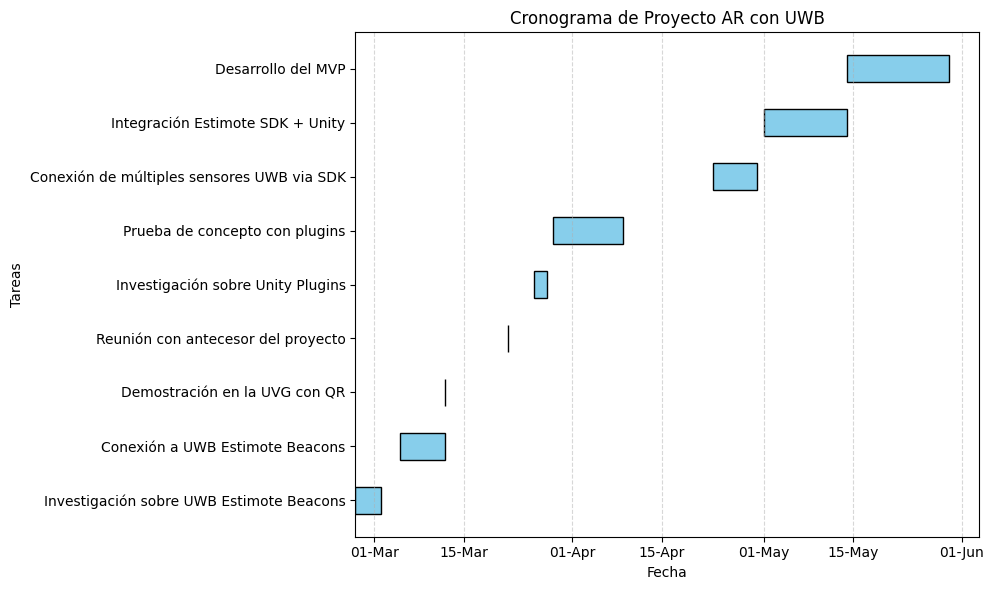
\includegraphics[width=1\textwidth]{images/cronograma.png}
{\begin{center}
    Figura 1: Cronograma del proyecto para el primer semestre.
\end{center}}
\newpage

    
 

\section{Bibliografía}
\begin{itemize} 
    % Bibliografia del marco teorico
    \item  Estimote, Inc. (n.d.). Estimote Proximity SDK. Estimote Documentation. Recuperado de: \url{https://developer.estimote.com/proximity/android-tutorial/}
    
    \item Estimote, Inc. (n.d.). Estimote Location Beacons: UWB and BLE. Estimote Documentation. Recuperado de: \url{https://developer.estimote.com/proximity/ultra-wideband/}
	
	\item Unity Technologies. (n.d.). AR Foundation overview. Unity Documentation. Recuperado de: \url{https://docs.unity3d.com/Packages/com.unity.xr.arfoundation@5.0/manual/index.html}
	
	\item Unity Technologies. (n.d.). Unity Manual: ARKit and ARCore with AR Foundation. Recuperado de: \url{https://docs.unity3d.com/Manual/com.unity.xr.arfoundation.html}
	
	\item Hart, P. E., Nilsson, N. J., \& Raphael, B. (1968). A formal basis for the heuristic determination of minimum cost paths. IEEE Transactions on Systems Science and Cybernetics, 4(2), 100–107. \url{https://doi.org/10.1109/TSSC.1968.300136}
	
	\item Thrun, S., Burgard, W., \& Fox, D. (2005). Probabilistic Robotics. MIT Press.
	
	\item Google. (n.d.). Bluetooth Low Energy overview | Android Developers. Recuperado de: \url{https://developer.android.com/guide/topics/connectivity/bluetooth-le}
	
	\item Apple Inc. (n.d.). Core Bluetooth Overview. Recuperado de: \url{https://developer.apple.com/documentation/corebluetooth}
\end{itemize}

\end{document}